\documentclass[floatfix,prb,aps,superscriptaddress,11pt,preprint,letterpaper]{revtex4}
\usepackage{amsfonts}
\usepackage{amsmath}
\usepackage{graphicx}
\allowdisplaybreaks[1]%biutiful equation breaker!!!
\usepackage{ulem}
\usepackage{subfigure}
%%%%%% defs
%%%% acronimos
\def\copyr{$^\copyright$}
\def\reg{\textsuperscript{\textregistered}}
\def\tm{\textsuperscript{\texttrademark}}
\def\lufac{LUFAC${^\textsuperscript{\textregistered}}$}
%\def\depe{DP${^\textsuperscript{\texttrademark}}$}
\def\depe{DP${\texttrademark}$}
\def\ps{\mathrm{ps}}
\def\lda{\mathrm{LDA}}
\def\rpa{\mathrm{RPA}}
\def\nl{\mathrm{nl}}
\def\acu{Accu-Check\textsuperscript{\textregistered}~Performa}
\def\goni{Glucometro \'Optico No Invasivo}
\def\Reg{\textsuperscript{\textregistered}}
\def\tiniba{TINIBA\textsuperscript{\textregistered}}
\def\gw{{\it GW}}
\def\gsa{Generaci\'on del Segundo Arm\'onico}
\def\shg{Second Harmonic Generation}
\def\sfg{Sum Frequency Generation}
\def\sdf{Generaci\'on de Suma de Frecuencias}
%%%%% accent of i
\def\'#1{\if#1i{\accent19\i}\else{\accent19#1}\fi}
%%%%% compa\~nias
\def\micro{{\it Supermicro}}
%%%%% lugares
\def\lou{Laboratorio de \'Optica Ultrar\'apida}
\def\roma{Universidad de Roma II}
\def\tor{``Tor Vergata''}
\def\dti{Direcci\'on de Tecnolog\'{\i}a e Innovaci\'on}
\def\dfa{Direcci\'on de Formaci\'on Acd\'emica}
\def\dg{Direcci\'on General}
\def\da{Direcci\'on Administrativa}
\def\ifug{Insituto de F\'isica de la U. de Guanajuato}
\def\icf{Instituto de Ciencias F\'isicas}
\def\unam{Universidad Nacional Aut\'onoma de M\'exico}
\def\uguille{Universidad del Nordeste, Argentina}
\def\fotonica{Departamento de Fotonica}
\def\grupo{Propiedades \'Opticas de Nano-Sistemas, Interfases y Superficies}
\def\grupoa{PRONASIS}
%\def\grupo{Propiedades \'Opticas de Superficies e Interfases y Sistemas Nanosc\'opicos}
%\def\grupoa{POSISNA}
\def\di{Direcci\'on de Investigaci\'on}
\def\dfa{Direcci\'on de Formaci\'on Acad\'emica}
\def\cio{Centro de Investigaciones en \'Optica}
\def\ciod{Centro de Investigaciones en \'Optica, León, Guanajuato.}
\def\Conacyt{Consejo Nacional de Ciencia y Tecnolog\'ia}
\def\Concyteg{Consejo  de Ciencia y Tecnolog\'ia del Estado de Guanajuato}
\def\conacyt{CONACyT}
\def\concyteg{CONCyTEG}
\def\lagos{Centro Universitario de los Lagos}
\def\udeg{Universidad de Guadalajara}
\def\dinv{Direcci\'on de Investigaci\'on}
\def\dop{Department of Physics}
\def\uoft{University of Toronto}
\def\ua{University of Texas at Austin}
\def\icf{Instituto de Ciencias Físicas, UNAM, Cuernavaca}
%%%%% gente
%% grupo
\def\gabriel{Gabriel Ramos Ortíz}
\def\ramon{Ram\'on~ Carriles~ Jaimes}
\def\ramonm{Ram\acute{o}n~ Carriles~ Jaimes}
\def\enrique{Enrique~ Castro~ Camus}
\def\raul{Ra\'ul Alfonso V\'azquez Nava}
\def\raulm{Ra\acute{u}l~ Alfonso~ V\acute{a}zquez~ Nava}
\def\beto{Norberto~ Arzate~ Plata}
\def\bmsa{Bernardo S. Mendoza}
\def\bms{Bernardo~ Mendoza~ Santoyo}
%% alumnos
\def\cesar{C\'esar Castillo Quevedo}
\def\cabellos{Jos\'e Luis Cabellos Quiroz}
\def\tona{Tonatiuh Rangel Gordillo}
\def\temok{Juan Cuauhtemoc Salazar Gonz\'alez}
\def\adan{Luis Adan Mart\'inez Jim\'enez}
\def\sean{Sean Martin Anderson}
\def\reinaldo{Reinaldo Zapata Pe\~na}
%%% alumnos del grupo
%% enrique
%Maestria:
\def\jorgee{Jorge Alberto Caballero Mendoza}
\def\sofia{Sofía Carolina Corzo García}
\def\ruth{Ruth Julieta Medina López} 
%Doctorado: 
\def\juane{Juan Jes\'us S\'anchez S\'anchez}
%Licenciatura
\def\alma{Alma Gabriela González Patlán}
%(con Ramon): 
\def\sergioer{Sergio Augusto Romero Serv\'{\i}n}
%% Raul
%Maestria:
\def\enriquer{Enrique Arag\'on Navarro}%udg
\def\salomonr{Salom\'on Rodr\'{\i}guez Carrera}
\def\hectorr{H\'ector Santiago Hern\'andez}
\def\victor{Victor Manuel Villanueva Reyes}
%% Ramon
%Maestria:
\def\alfredora{Alfredo Campos Mej\'{\i}a}
%% Beto
%Doctorado
\def\noe{No\'e Gonz\'alez Baquedano}
%% otros
\def\liliana{Liliana Wilson Herr\'an}
\def\gerardo{Gerardo E. S\'anchez Garc\'{\i}a Rojas}
\def\amalia{Amalia Mart\'inez Garc\'{\i}a}
\def\nacho{Ing. José Ignacio Diego Manrique}
\def\tere{Teresita del Niño Jesús Pérez Hernández}
\def\elder{Elder de la Rosa Cruz}
\def\gonzalo{Gonzalo P\'aez Padilla}
\def\wlm{W. Luis Moch\'an Backal}
\def\oracio{Oracio C. Barbosa Garc\'ia}
\def\hector{H\'ector Hugo S\'anchez Hern\'andez}
\def\marco{Marco Antonio Escobar-Acevedo}
\def\gil{Alejandro Gil-Villegas Montiel}
\def\ernesto{Ernesto Carlos Cort\'es Morales}
\def\fms{Fernando Mendoza Santoyo}
\def\cuevas{Francisco Javier Cuevas de la Rosa}
\def\brenda{Brenda Esmeralda Matr\'inez Z\'erega}
\def\guille{Guillermo Ortiz}
\def\cesar{Cesar Castillo Quevedo}
\def\sipe{Prof. John Sipe}
\def\mike{Prof. Michael Downer}
\def\jems{Jorge Enrique Mej\'ia S\'anchez}
\def\lamon{Ram\'on Rodr\'iguez Vera}
\def\ldp{Luis de la Pe\~na}
\def\sole{Rodolfo Del Sole}
\def\lucia{Lucia Reining}
\def\sch{Schr\"odinger}
\def\Cuevas{Francisco J. Cuevas de la Rosa}
%%%%% categorias
\def\ita{Investigador Titular A}
\def\itb{Investigador Titular B}
\def\itc{Investigador Titular C}
\def\itd{Investigador Titular D}
\def\ite{Investigador Titular E}
\def\sr{Senior Researcher}
\def\iac{Investigador Asociado C}    
\def\alm{Alumno de Maestr\'ia}
\def\ald{Alumno de Doctorado}
\def\all{Alumno de Licenciatura}
\def\adei{Asistente de Investigaci\'on}
\def\sniIII{S.N.I. nivel III}
\def\sni{S.N.I.}
\def\cv{Currículum Vitae}
%%%%%% fonts
\def\tit{\sf}
\def\col{\sc}
\def\alu{\it} % for students
\def\cual{2$^{do}$}
\def\anno{2005}
\def\spe{\vspace{.12cm}}
%%%%%% cosas
\def\capa{capa-a-capa}
\def\espin{espintr\'onica}
\def\oespin{optoespintr\'onica}
\def\proyecto{Photon Assisted Spintronics}
\def\npro{48915}
\def\cvk{cv\mathbf{k}}
\def\cvkp{c'v'\mathbf{k}'}
%%%%%% revistas
\def\prb{Physical Review B}
\def\prl{Physical Review Letters}
\def\ol{Optics Letters}
\def\opn{Optics and Photonics News}
\def\pssc{physica status solidi (c)}
%%%%%%%%%%%%%%%%%%%%%%%%%%%%%%%%%%%%%%%
%%%%%% griegas
\def\ga{\alpha}
\def\gb{\beta}
\def\gga{\gamma}
\def\gGa{\Gamma}
\def\go{\omega}
\def\got{\tilde\omega}
\def\gO{\Omega}
\def\gr{{\rho}}
\def\ge{\epsilon}
\def\ve{\varepsilon}
\def\gve{\varepsilon}
\def\gd{\delta}
\def\gD{\Delta}
\def\gl{\lambda}
\def\gs{\sigma}
\def\gS{\Sigma}
\def\gbs{\overline{\sigma}}
\def\gka{\kappa}
%%%%%% griegas with tilde
\def\gta{\tilde{\alpha}}
\def\gtb{\tilde{\beta}}
\def\gtga{\tilde{\gamma}}
\def\gto{\tilde{\omega}}
\def\gtO{\tilde{\Omega}}
\def\gtr{\tilde{\rho}}
\def\gte{\tilde{\epsilon}}
\def\vte{\tilde{\varepsilon}}
\def\gtd{\tilde{\delta}}
\def\gtD{\tilde{\Delta}}
\def\gtl{\tilde{\lambda}}
\def\gts{\tilde{\sigma}}
\def\gtS{\tilde{\Sigma}}
%%%%%% romans with tilde
\def\bftr{\tilde{\mathbf{r}}}
\def\bftp{\tilde{\mathbf{p}}}
\def\bftv{\tilde{\mathbf{v}}}
\def\ta{\tilde{a}}
\def\tb{\tilde{b}}
\def\tr{\tilde{r}}
\def\tp{\tilde{p}}
\def\tV{\tilde{V}}
\def\tv{\tilde{v}}
%%
\newcommand{\ham}{\hat{\mathcal H}}
%%%%%% bra kets
\newcommand{\la}{\langle}
\newcommand{\ra}{\rangle}
\newcommand{\ket}[1]{| #1 \rangle}
\newcommand{\bra}[1]{\langle #1 |}
\newcommand{\braket}[2]{\langle {#1} | {#2} \rangle}
\newcommand{\ketbra}[2]{| {#1} \rangle {#1} \langle {#2} |}
\newcommand{\ave}[1]{\langle {#1} \rangle}
\newcommand{\dotp}[2]{\mathbf{#1} \cdot \mathbf{#2}}
%%%%%% averages
\newcommand{\prom}[1]{\langle {#1} \rangle}
%%%%%% creation and annihilation operators
\newcommand{\oa}{\hat a^{\tiny\strut}}
\newcommand{\oad}{\hat a^\dagger}
\newcommand{\oadk}{\hat a^\dagger_{\mathbf k}}
\newcommand{\oak}{\hat a^{\tiny\strut}_{\mathbf k}}
\newcommand{\obd}[1]{\hat b^\dagger_{#1}}
\newcommand{\ob}[1]{\hat b^{\tiny\strut}_{#1}}
%%%%%% Caligraphic
\newcommand{\cala}{{\mathbf{\cal A}}}
\newcommand{\calb}{{\mathbf{\cal B}}}
\newcommand{\calc}{{\mathbf{\cal C}}}
\newcommand{\cald}{{\mathbf{\cal D}}}
\newcommand{\cale}{{\mathbf{\cal E}}}
\newcommand{\calf}{{\mathbf{\cal F}}}
\newcommand{\calh}{{\mathbf{\cal H}}}
\newcommand{\cali}{{\mathbf{\cal I}}}
\newcommand{\calp}{{\mathbf{\cal P}}}
\newcommand{\calg}{{\mathbf{\cal G}}}
\newcommand{\calv}{{\mathbf{\cal V}}}
\newcommand{\call}{{\cal L}}
\newcommand{\calo}{{\cal O}}
\newcommand{\caln}{{\cal N}}
\newcommand{\calr}{{\cal R}}
\newcommand{\cals}{{\cal S}}
\newcommand{\calt}{{\cal T}}
\newcommand{\calu}{{\cal U}}
\newcommand{\calw}{{\cal W}}
\newcommand{\calbd}{\boldsymbol{\mathcal{\cal D}}}
\newcommand{\calbp}{\boldsymbol{\mathcal{\cal P}}}
\newcommand{\calbv}{\boldsymbol{\mathcal{\cal V}}}
\newcommand{\calbs}{\boldsymbol{\mathcal{\cal S}}}
\newcommand{\calbg}{\boldsymbol{\mathcal{\cal G}}}
%%%%%% mathematicla bold roman & greek
\newcommand{\mbf}[1]{\mathbf{#1}}
\newcommand{\mbg}[1]{\boldsymbol{\mathcal {#1}}}
\newcommand{\bfA}{\mathbf{A}}
\newcommand{\bfB}{\mathbf{B}}
\newcommand{\bfC}{\mathbf{C}}
\newcommand{\bfD}{\mathbf{D}}
\newcommand{\bfE}{\mathbf{E}}
\newcommand{\bfF}{\mathbf{F}}
\newcommand{\bfG}{\mathbf{G}}
\newcommand{\bfH}{\mathbf{H}}
\newcommand{\bfI}{\mathbf{I}}
\newcommand{\bfJ}{\mathbf{J}}
\newcommand{\bfK}{\mathbf{K}}
\newcommand{\bfL}{\mathbf{L}}
\newcommand{\bfM}{\mathbf{M}}
\newcommand{\bfN}{\mathbf{N}}
\newcommand{\bfP}{\mathbf{P}}
\newcommand{\bfR}{\mathbf{R}}
\newcommand{\bfS}{\mathbf{S}}
\newcommand{\bfT}{\mathbf{T}}
\newcommand{\bfU}{\mathbf{U}}
\newcommand{\bfV}{\mathbf{V}}
\newcommand{\bfW}{\mathbf{W}}
\newcommand{\bfX}{\mathbf{X}}
\newcommand{\bfY}{\mathbf{Y}}
\newcommand{\bfZ}{\mathbf{Z}}
\newcommand{\bfa}{\mathbf{a}}
\newcommand{\bfb}{\mathbf{b}}
\newcommand{\bfc}{\mathbf{c}}
\newcommand{\bfd}{\mathbf{d}}
\newcommand{\bfe}{\mathbf{e}}
\newcommand{\bff}{\mathbf{f}}
\newcommand{\bfg}{\mathbf{g}}
\newcommand{\bfh}{\mathbf{h}}
\newcommand{\bfi}{\mathbf{i}}
\newcommand{\bfj}{\mathbf{j}}
\newcommand{\bfk}{\mathbf{k}}
\newcommand{\bfn}{\mathbf{n}}
\newcommand{\bfp}{\mathbf{p}}
\newcommand{\bfq}{\mathbf{q}}
\newcommand{\bfr}{\mathbf{r}}
\newcommand{\bfs}{\mathbf{s}}
\newcommand{\bft}{\mathbf{t}}
\newcommand{\bfu}{\mathbf{u}}
\newcommand{\bfv}{\mathbf{v}}
\newcommand{\bfx}{\mathbf{x}}
\newcommand{\bfy}{\mathbf{y}}
\newcommand{\bfz}{\mathbf{z}}
\newcommand{\bfzero}{\mathbf{0}}
\newcommand{\bfone}{\mathbf{1}}
%
\newcommand{\bfgeta}{\boldsymbol{\eta}}
\newcommand{\bfSig}{\boldsymbol{\Sigma}}
\newcommand{\bfsig}{\boldsymbol{\sigma}}
\newcommand{\bfgS}{\boldsymbol{\Sigma}}
\newcommand{\bfgs}{\boldsymbol{\sigma}}
\newcommand{\bfga}{\boldsymbol{\alpha}}
\newcommand{\bfgb}{\boldsymbol{\beta}}
\newcommand{\bfge}{\boldsymbol{\epsilon}}
\newcommand{\bfgvare}{\boldsymbol{\varepsilon}}
\newcommand{\bfgg}{\boldsymbol{\gamma}}
\newcommand{\bfgG}{\boldsymbol{\Gamma}}
\newcommand{\bfgphi}{\boldsymbol{\phi}}
\newcommand{\bfgpsi}{\boldsymbol{\psi}}
\newcommand{\bfgD}{\boldsymbol{\Delta}}
\newcommand{\bfgPhi}{\boldsymbol{\Phi}}
\newcommand{\bfgPsi}{\boldsymbol{\Psi}}
\newcommand{\bfgtau}{\boldsymbol{\tau}}
\newcommand{\bfgxi}{\boldsymbol{\xi}}
\newcommand{\bfgchi}{\boldsymbol{\chi}}
\newcommand{\bfgnabla}{\boldsymbol{\nabla}}
\newcommand{\bfgnu}{\boldsymbol{\nu}}
\newcommand{\bfgmu}{\boldsymbol{\mu}}
\newcommand{\bfgrho}{\boldsymbol{\rho}}
\newcommand{\bfgRho}{\boldsymbol{\Rho}}
%%%%%% nabla
\newcommand{\nablak}{\frac{\partial}{\partial\mathbf{k}} }
%%%%%% ; derivative
\def\gk{{;\mathbf k}}
%%%%%% k derivative
\newcommand{\deriv}[2] {\frac{\partial {#1}} {\partial {#2} }}
%%%%%% prime for \sum
\def\prima{\strut^{_{'}}}
%%%%%% subindices
%\def\eti{n\bfk}
\newcommand{\eti}[1]{_{#1 \bfk}}
\newcommand{\etiup}[1]{_{#1 \bfk s}}
\newcommand{\etidn}[1]{_{#1 \bfk \bar{s}}}
%%%%% superindice to push down the subindex in greeks!
\def\pd{^{\strut}}
%%%%% gauges
\def\rde{$\bfr\cdot\bfE$~}
\def\rder{length-gauge}
\def\pda{$\bfp\cdot\bfA$~}
\def\vda{$\bfv\cdot\bfA$~}
\def\vdar{velocity-gauge}
%%%%% integral over k
\def\intk{\int\frac{d^3k}{8\pi^3}}
%%%%% roman indices
\def\rmi{\mathrm{i}}
\def\rmj{\mathrm{j}}
\def\rmk{\mathrm{k}}
\def\rml{\mathrm{l}}
\def\rmr{\mathrm{r}}
\def\rma{\mathrm{a}}
\def\rmb{\mathrm{b}}
\def\rmc{\mathrm{c}}
\def\rmd{\mathrm{d}}
\def\rme{\mathrm{e}}
\def\rmv{\mathrm{v}}
\def\rmz{\mathrm{z}}
\def\rmx{\mathrm{x}}
\def\rmy{\mathrm{y}}
\def\rmH{\mathrm{H}}
\def\rmI{\mathrm{I}}
\def\rmG{\mathrm{G}}
\def\rmW{\mathrm{W}}
%%%%% functions
\def\erf{\mathrm{erf}}
\def\erfc{\mathrm{erfc}}
\def\erfi{\mathrm{erfi}}

%iave: C01243171 y 0124317111
%%%%% Green's one point model
\def\tyv{\tilde y_v}
\def\ty{\tilde y}
\def\tv{\tilde v}

%%%%% defs
%%%% acronimos
\def\copyr{$^\copyright$}
\def\reg{\textsuperscript{\textregistered}}
\def\tm{\textsuperscript{\texttrademark}}
\def\lufac{LUFAC${^\textsuperscript{\textregistered}}$}
%\def\depe{DP${^\textsuperscript{\texttrademark}}$}
\def\depe{DP${\texttrademark}$}
\def\ps{\mathrm{ps}}
\def\lda{\mathrm{LDA}}
\def\rpa{\mathrm{RPA}}
\def\nl{\mathrm{nl}}
\def\acu{Accu-Check\textsuperscript{\textregistered}~Performa}
\def\goni{Glucometro \'Optico No Invasivo}
\def\Reg{\textsuperscript{\textregistered}}
\def\tiniba{TINIBA\textsuperscript{\textregistered}}
\def\gw{{\it GW}}
\def\gsa{Generaci\'on del Segundo Arm\'onico}
\def\shg{Second Harmonic Generation}
\def\sfg{Sum Frequency Generation}
\def\sdf{Generaci\'on de Suma de Frecuencias}
%%%%% accent of i
\def\'#1{\if#1i{\accent19\i}\else{\accent19#1}\fi}
%%%%% compa\~nias
\def\micro{{\it Supermicro}}
%%%%% lugares
\def\lou{Laboratorio de \'Optica Ultrar\'apida}
\def\roma{Universidad de Roma II}
\def\tor{``Tor Vergata''}
\def\dti{Direcci\'on de Tecnolog\'{\i}a e Innovaci\'on}
\def\dfa{Direcci\'on de Formaci\'on Acd\'emica}
\def\dg{Direcci\'on General}
\def\da{Direcci\'on Administrativa}
\def\ifug{Insituto de F\'isica de la U. de Guanajuato}
\def\icf{Instituto de Ciencias F\'isicas}
\def\unam{Universidad Nacional Aut\'onoma de M\'exico}
\def\uguille{Universidad del Nordeste, Argentina}
\def\fotonica{Departamento de Fotonica}
\def\grupo{Propiedades \'Opticas de Nano-Sistemas, Interfases y Superficies}
\def\grupoa{PRONASIS}
%\def\grupo{Propiedades \'Opticas de Superficies e Interfases y Sistemas Nanosc\'opicos}
%\def\grupoa{POSISNA}
\def\di{Direcci\'on de Investigaci\'on}
\def\dfa{Direcci\'on de Formaci\'on Acad\'emica}
\def\cio{Centro de Investigaciones en \'Optica}
\def\ciod{Centro de Investigaciones en \'Optica, León, Guanajuato.}
\def\Conacyt{Consejo Nacional de Ciencia y Tecnolog\'ia}
\def\Concyteg{Consejo  de Ciencia y Tecnolog\'ia del Estado de Guanajuato}
\def\conacyt{CONACyT}
\def\concyteg{CONCyTEG}
\def\lagos{Centro Universitario de los Lagos}
\def\udeg{Universidad de Guadalajara}
\def\dinv{Direcci\'on de Investigaci\'on}
\def\dop{Department of Physics}
\def\uoft{University of Toronto}
\def\ua{University of Texas at Austin}
\def\icf{Instituto de Ciencias Físicas, UNAM, Cuernavaca}
%%%%% gente
%% grupo
\def\gabriel{Gabriel Ramos Ortíz}
\def\ramon{Ram\'on~ Carriles~ Jaimes}
\def\ramonm{Ram\acute{o}n~ Carriles~ Jaimes}
\def\enrique{Enrique~ Castro~ Camus}
\def\raul{Ra\'ul Alfonso V\'azquez Nava}
\def\raulm{Ra\acute{u}l~ Alfonso~ V\acute{a}zquez~ Nava}
\def\beto{Norberto~ Arzate~ Plata}
\def\bmsa{Bernardo S. Mendoza}
\def\bms{Bernardo~ Mendoza~ Santoyo}
%% alumnos
\def\cesar{C\'esar Castillo Quevedo}
\def\cabellos{Jos\'e Luis Cabellos Quiroz}
\def\tona{Tonatiuh Rangel Gordillo}
\def\temok{Juan Cuauhtemoc Salazar Gonz\'alez}
\def\adan{Luis Adan Mart\'inez Jim\'enez}
\def\sean{Sean Martin Anderson}
\def\reinaldo{Reinaldo Zapata Pe\~na}
%%% alumnos del grupo
%% enrique
%Maestria:
\def\jorgee{Jorge Alberto Caballero Mendoza}
\def\sofia{Sofía Carolina Corzo García}
\def\ruth{Ruth Julieta Medina López} 
%Doctorado: 
\def\juane{Juan Jes\'us S\'anchez S\'anchez}
%Licenciatura
\def\alma{Alma Gabriela González Patlán}
%(con Ramon): 
\def\sergioer{Sergio Augusto Romero Serv\'{\i}n}
%% Raul
%Maestria:
\def\enriquer{Enrique Arag\'on Navarro}%udg
\def\salomonr{Salom\'on Rodr\'{\i}guez Carrera}
\def\hectorr{H\'ector Santiago Hern\'andez}
\def\victor{Victor Manuel Villanueva Reyes}
%% Ramon
%Maestria:
\def\alfredora{Alfredo Campos Mej\'{\i}a}
%% Beto
%Doctorado
\def\noe{No\'e Gonz\'alez Baquedano}
%% otros
\def\liliana{Liliana Wilson Herr\'an}
\def\gerardo{Gerardo E. S\'anchez Garc\'{\i}a Rojas}
\def\amalia{Amalia Mart\'inez Garc\'{\i}a}
\def\nacho{Ing. José Ignacio Diego Manrique}
\def\tere{Teresita del Niño Jesús Pérez Hernández}
\def\elder{Elder de la Rosa Cruz}
\def\gonzalo{Gonzalo P\'aez Padilla}
\def\wlm{W. Luis Moch\'an Backal}
\def\oracio{Oracio C. Barbosa Garc\'ia}
\def\hector{H\'ector Hugo S\'anchez Hern\'andez}
\def\marco{Marco Antonio Escobar-Acevedo}
\def\gil{Alejandro Gil-Villegas Montiel}
\def\ernesto{Ernesto Carlos Cort\'es Morales}
\def\fms{Fernando Mendoza Santoyo}
\def\cuevas{Francisco Javier Cuevas de la Rosa}
\def\brenda{Brenda Esmeralda Matr\'inez Z\'erega}
\def\guille{Guillermo Ortiz}
\def\cesar{Cesar Castillo Quevedo}
\def\sipe{Prof. John Sipe}
\def\mike{Prof. Michael Downer}
\def\jems{Jorge Enrique Mej\'ia S\'anchez}
\def\lamon{Ram\'on Rodr\'iguez Vera}
\def\ldp{Luis de la Pe\~na}
\def\sole{Rodolfo Del Sole}
\def\lucia{Lucia Reining}
\def\sch{Schr\"odinger}
\def\Cuevas{Francisco J. Cuevas de la Rosa}
%%%%% categorias
\def\ita{Investigador Titular A}
\def\itb{Investigador Titular B}
\def\itc{Investigador Titular C}
\def\itd{Investigador Titular D}
\def\ite{Investigador Titular E}
\def\sr{Senior Researcher}
\def\iac{Investigador Asociado C}    
\def\alm{Alumno de Maestr\'ia}
\def\ald{Alumno de Doctorado}
\def\all{Alumno de Licenciatura}
\def\adei{Asistente de Investigaci\'on}
\def\sniIII{S.N.I. nivel III}
\def\sni{S.N.I.}
\def\cv{Currículum Vitae}
%%%%%% fonts
\def\tit{\sf}
\def\col{\sc}
\def\alu{\it} % for students
\def\cual{2$^{do}$}
\def\anno{2005}
\def\spe{\vspace{.12cm}}
%%%%%% cosas
\def\capa{capa-a-capa}
\def\espin{espintr\'onica}
\def\oespin{optoespintr\'onica}
\def\proyecto{Photon Assisted Spintronics}
\def\npro{48915}
\def\cvk{cv\mathbf{k}}
\def\cvkp{c'v'\mathbf{k}'}
%%%%%% revistas
\def\prb{Physical Review B}
\def\prl{Physical Review Letters}
\def\ol{Optics Letters}
\def\opn{Optics and Photonics News}
\def\pssc{physica status solidi (c)}
%%%%%%%%%%%%%%%%%%%%%%%%%%%%%%%%%%%%%%%
%%%%%% griegas
\def\ga{\alpha}
\def\gb{\beta}
\def\gga{\gamma}
\def\gGa{\Gamma}
\def\go{\omega}
\def\got{\tilde\omega}
\def\gO{\Omega}
\def\gr{{\rho}}
\def\ge{\epsilon}
\def\ve{\varepsilon}
\def\gve{\varepsilon}
\def\gd{\delta}
\def\gD{\Delta}
\def\gl{\lambda}
\def\gs{\sigma}
\def\gS{\Sigma}
\def\gbs{\overline{\sigma}}
\def\gka{\kappa}
%%%%%% griegas with tilde
\def\gta{\tilde{\alpha}}
\def\gtb{\tilde{\beta}}
\def\gtga{\tilde{\gamma}}
\def\gto{\tilde{\omega}}
\def\gtO{\tilde{\Omega}}
\def\gtr{\tilde{\rho}}
\def\gte{\tilde{\epsilon}}
\def\vte{\tilde{\varepsilon}}
\def\gtd{\tilde{\delta}}
\def\gtD{\tilde{\Delta}}
\def\gtl{\tilde{\lambda}}
\def\gts{\tilde{\sigma}}
\def\gtS{\tilde{\Sigma}}
%%%%%% romans with tilde
\def\bftr{\tilde{\mathbf{r}}}
\def\bftp{\tilde{\mathbf{p}}}
\def\bftv{\tilde{\mathbf{v}}}
\def\ta{\tilde{a}}
\def\tb{\tilde{b}}
\def\tr{\tilde{r}}
\def\tp{\tilde{p}}
\def\tV{\tilde{V}}
\def\tv{\tilde{v}}
%%
\newcommand{\ham}{\hat{\mathcal H}}
%%%%%% bra kets
\newcommand{\la}{\langle}
\newcommand{\ra}{\rangle}
\newcommand{\ket}[1]{| #1 \rangle}
\newcommand{\bra}[1]{\langle #1 |}
\newcommand{\braket}[2]{\langle {#1} | {#2} \rangle}
\newcommand{\ketbra}[2]{| {#1} \rangle {#1} \langle {#2} |}
\newcommand{\ave}[1]{\langle {#1} \rangle}
\newcommand{\dotp}[2]{\mathbf{#1} \cdot \mathbf{#2}}
%%%%%% averages
\newcommand{\prom}[1]{\langle {#1} \rangle}
%%%%%% creation and annihilation operators
\newcommand{\oa}{\hat a^{\tiny\strut}}
\newcommand{\oad}{\hat a^\dagger}
\newcommand{\oadk}{\hat a^\dagger_{\mathbf k}}
\newcommand{\oak}{\hat a^{\tiny\strut}_{\mathbf k}}
\newcommand{\obd}[1]{\hat b^\dagger_{#1}}
\newcommand{\ob}[1]{\hat b^{\tiny\strut}_{#1}}
%%%%%% Caligraphic
\newcommand{\cala}{{\mathbf{\cal A}}}
\newcommand{\calb}{{\mathbf{\cal B}}}
\newcommand{\calc}{{\mathbf{\cal C}}}
\newcommand{\cald}{{\mathbf{\cal D}}}
\newcommand{\cale}{{\mathbf{\cal E}}}
\newcommand{\calf}{{\mathbf{\cal F}}}
\newcommand{\calh}{{\mathbf{\cal H}}}
\newcommand{\cali}{{\mathbf{\cal I}}}
\newcommand{\calp}{{\mathbf{\cal P}}}
\newcommand{\calg}{{\mathbf{\cal G}}}
\newcommand{\calv}{{\mathbf{\cal V}}}
\newcommand{\call}{{\cal L}}
\newcommand{\calo}{{\cal O}}
\newcommand{\caln}{{\cal N}}
\newcommand{\calr}{{\cal R}}
\newcommand{\cals}{{\cal S}}
\newcommand{\calt}{{\cal T}}
\newcommand{\calu}{{\cal U}}
\newcommand{\calw}{{\cal W}}
\newcommand{\calbd}{\boldsymbol{\mathcal{\cal D}}}
\newcommand{\calbp}{\boldsymbol{\mathcal{\cal P}}}
\newcommand{\calbv}{\boldsymbol{\mathcal{\cal V}}}
\newcommand{\calbs}{\boldsymbol{\mathcal{\cal S}}}
\newcommand{\calbg}{\boldsymbol{\mathcal{\cal G}}}
%%%%%% mathematicla bold roman & greek
\newcommand{\mbf}[1]{\mathbf{#1}}
\newcommand{\mbg}[1]{\boldsymbol{\mathcal {#1}}}
\newcommand{\bfA}{\mathbf{A}}
\newcommand{\bfB}{\mathbf{B}}
\newcommand{\bfC}{\mathbf{C}}
\newcommand{\bfD}{\mathbf{D}}
\newcommand{\bfE}{\mathbf{E}}
\newcommand{\bfF}{\mathbf{F}}
\newcommand{\bfG}{\mathbf{G}}
\newcommand{\bfH}{\mathbf{H}}
\newcommand{\bfI}{\mathbf{I}}
\newcommand{\bfJ}{\mathbf{J}}
\newcommand{\bfK}{\mathbf{K}}
\newcommand{\bfL}{\mathbf{L}}
\newcommand{\bfM}{\mathbf{M}}
\newcommand{\bfN}{\mathbf{N}}
\newcommand{\bfP}{\mathbf{P}}
\newcommand{\bfR}{\mathbf{R}}
\newcommand{\bfS}{\mathbf{S}}
\newcommand{\bfT}{\mathbf{T}}
\newcommand{\bfU}{\mathbf{U}}
\newcommand{\bfV}{\mathbf{V}}
\newcommand{\bfW}{\mathbf{W}}
\newcommand{\bfX}{\mathbf{X}}
\newcommand{\bfY}{\mathbf{Y}}
\newcommand{\bfZ}{\mathbf{Z}}
\newcommand{\bfa}{\mathbf{a}}
\newcommand{\bfb}{\mathbf{b}}
\newcommand{\bfc}{\mathbf{c}}
\newcommand{\bfd}{\mathbf{d}}
\newcommand{\bfe}{\mathbf{e}}
\newcommand{\bff}{\mathbf{f}}
\newcommand{\bfg}{\mathbf{g}}
\newcommand{\bfh}{\mathbf{h}}
\newcommand{\bfi}{\mathbf{i}}
\newcommand{\bfj}{\mathbf{j}}
\newcommand{\bfk}{\mathbf{k}}
\newcommand{\bfn}{\mathbf{n}}
\newcommand{\bfp}{\mathbf{p}}
\newcommand{\bfq}{\mathbf{q}}
\newcommand{\bfr}{\mathbf{r}}
\newcommand{\bfs}{\mathbf{s}}
\newcommand{\bft}{\mathbf{t}}
\newcommand{\bfu}{\mathbf{u}}
\newcommand{\bfv}{\mathbf{v}}
\newcommand{\bfx}{\mathbf{x}}
\newcommand{\bfy}{\mathbf{y}}
\newcommand{\bfz}{\mathbf{z}}
\newcommand{\bfzero}{\mathbf{0}}
\newcommand{\bfone}{\mathbf{1}}
%
\newcommand{\bfgeta}{\boldsymbol{\eta}}
\newcommand{\bfSig}{\boldsymbol{\Sigma}}
\newcommand{\bfsig}{\boldsymbol{\sigma}}
\newcommand{\bfgS}{\boldsymbol{\Sigma}}
\newcommand{\bfgs}{\boldsymbol{\sigma}}
\newcommand{\bfga}{\boldsymbol{\alpha}}
\newcommand{\bfgb}{\boldsymbol{\beta}}
\newcommand{\bfge}{\boldsymbol{\epsilon}}
\newcommand{\bfgvare}{\boldsymbol{\varepsilon}}
\newcommand{\bfgg}{\boldsymbol{\gamma}}
\newcommand{\bfgG}{\boldsymbol{\Gamma}}
\newcommand{\bfgphi}{\boldsymbol{\phi}}
\newcommand{\bfgpsi}{\boldsymbol{\psi}}
\newcommand{\bfgD}{\boldsymbol{\Delta}}
\newcommand{\bfgPhi}{\boldsymbol{\Phi}}
\newcommand{\bfgPsi}{\boldsymbol{\Psi}}
\newcommand{\bfgtau}{\boldsymbol{\tau}}
\newcommand{\bfgxi}{\boldsymbol{\xi}}
\newcommand{\bfgchi}{\boldsymbol{\chi}}
\newcommand{\bfgnabla}{\boldsymbol{\nabla}}
\newcommand{\bfgnu}{\boldsymbol{\nu}}
\newcommand{\bfgmu}{\boldsymbol{\mu}}
\newcommand{\bfgrho}{\boldsymbol{\rho}}
\newcommand{\bfgRho}{\boldsymbol{\Rho}}
%%%%%% nabla
\newcommand{\nablak}{\frac{\partial}{\partial\mathbf{k}} }
%%%%%% ; derivative
\def\gk{{;\mathbf k}}
%%%%%% k derivative
\newcommand{\deriv}[2] {\frac{\partial {#1}} {\partial {#2} }}
%%%%%% prime for \sum
\def\prima{\strut^{_{'}}}
%%%%%% subindices
%\def\eti{n\bfk}
\newcommand{\eti}[1]{_{#1 \bfk}}
\newcommand{\etiup}[1]{_{#1 \bfk s}}
\newcommand{\etidn}[1]{_{#1 \bfk \bar{s}}}
%%%%% superindice to push down the subindex in greeks!
\def\pd{^{\strut}}
%%%%% gauges
\def\rde{$\bfr\cdot\bfE$~}
\def\rder{length-gauge}
\def\pda{$\bfp\cdot\bfA$~}
\def\vda{$\bfv\cdot\bfA$~}
\def\vdar{velocity-gauge}
%%%%% integral over k
\def\intk{\int\frac{d^3k}{8\pi^3}}
%%%%% roman indices
\def\rmi{\mathrm{i}}
\def\rmj{\mathrm{j}}
\def\rmk{\mathrm{k}}
\def\rml{\mathrm{l}}
\def\rmr{\mathrm{r}}
\def\rma{\mathrm{a}}
\def\rmb{\mathrm{b}}
\def\rmc{\mathrm{c}}
\def\rmd{\mathrm{d}}
\def\rme{\mathrm{e}}
\def\rmv{\mathrm{v}}
\def\rmz{\mathrm{z}}
\def\rmx{\mathrm{x}}
\def\rmy{\mathrm{y}}
\def\rmH{\mathrm{H}}
\def\rmI{\mathrm{I}}
\def\rmG{\mathrm{G}}
\def\rmW{\mathrm{W}}
%%%%% functions
\def\erf{\mathrm{erf}}
\def\erfc{\mathrm{erfc}}
\def\erfi{\mathrm{erfi}}

%iave: C01243171 y 0124317111
%%%%% Green's one point model
\def\tyv{\tilde y_v}
\def\ty{\tilde y}
\def\tv{\tilde v}

\usepackage{bm}
%%%%*****************%%%% fine hyperef 
\usepackage[backref,pdffitwindow,colorlinks,linkcolor={blue},citecolor={red}]{hyperref}
%%%%%%%%%%%%%%%%%%%%%%%%%%%%%%%%%%%%%%%
\usepackage{showlabels}
%\usepackage{showkeys}


\begin{document}

\title{Length Gauge Theory of Surface Second Harmonic Generation}
\author{Sean M. Anderson}
\affiliation{Centro de Investigaciones en Optica, Le\'on, Guanajuato, M\'exico}
\author{Nicolas Tancogne-Dejean}
\affiliation{Laboratoire des Solides Irradi\'es, \'Ecole 
  Polytechnique, CNRS, CEA/DSM, 91128 Palaiseau, France}
 \affiliation{European Theoretical Spectroscopy Facility (ETSF), Palaiseau, France}
\author{Bernardo S. Mendoza}\email{bms@cio.mx}
\affiliation{Centro de Investigaciones en Optica, Le\'on, Guanajuato, M\'exico}
\author{Val\'erie V\'eniard}
\affiliation{Laboratoire des Solides Irradi\'es, \'Ecole 
  Polytechnique, CNRS, CEA/DSM, 91128 Palaiseau, France}
 \affiliation{European Theoretical Spectroscopy Facility (ETSF), Palaiseau, France}

\begin{abstract}
We present a theoretical review of surface second harmonic generation (SHG) 
from semiconductor surfaces based on the longitudinal gauge. This 
layer-by-layer analysis is carefully presented in order to show how a 
surface SHG calculation can be readily evaluated. The nonlinear susceptibility 
tensor for a surface, $\boldsymbol{\chi}^S(-2\go;\go,\go)$
 is split into two terms relating to inter-band 
and intra-band one-electron transitions. 

\end{abstract}  

\maketitle
%\tableofcontents

\section{Theory}

\label{theory}

In this section we present the scheme used to calculate the surface second-order
nonlinear response.
Our derivation includes new terms not included
before in the length gauge formalism for the surface nonlinear
response. 

\subsection{Perturbation approach}

We use the independent particle approximation and neglect local field
and excitonic effects and
treat the electromagnetic field classically, while the matter is
described quantum-mechanically.
We can describe the system using 
%a scaled 
the one electron density
operator ${\rho}$, with which we can calculate the expectation value of a
single-particle observable $\mathcal{O}$ as 
$\langle{\cal O}\rangle=\mbox{Tr}({\rho} {\cal O}),  
\label{calo}$
with $\mathcal{O}$ the associated quantum mechanical operator and Tr
the trace. 
The density operator satisfies
$
i\hbar (d{\rho}/dt)=[H(t),{\rho}],  
\label{rho}
$
with $H(t)$ as the total single electron Hamiltonian, written as 
\begin{equation*}
H(t)=H_{0}+H_{I}(t),  
\label{ache}
\end{equation*}
where $H_{0}$ is the unperturbed time-independent Hamiltonian, and $H_{I}(t)$
is the time-dependent potential energy due to the interaction of the
electron with the electromagnetic field.
% ; $H_{0}$ has eigenvalues
% $\hbar \omega_{n}(\mathbf{k})$
% and eigenstates $| n\mathbf{k} \rangle$ (Bloch states) labeled by a band 
% index $n$ and crystal momentum $\mathbf{k}$.
To proceed with the solution of $\rho$  it is convenient to use the
interaction picture, where a unitary operator $U=\exp ({iH_{0}t/\hbar })$
transforms any operator $\mathcal{O}$ into 
$\tilde{\mathcal{O}}=U{\cal O}U^{\dagger }$. Even if $\mathcal{O}$ does not depend on $t$, $\tilde{
\mathcal{O}}$ does through the explicit time dependence of $U$. 
The dynamical 
equation for $\tilde{\rho}$ is 
given by
\begin{equation*}
i\hbar \frac{d\tilde{{\rho}}}{dt}=[\tilde{H}_{I}(t),\tilde{{\rho}}],  
\label{rho1}
\end{equation*}
with solution 
\begin{equation}
i\hbar \tilde{{\rho}}(t)=i\hbar \tilde{{\rho}}_{0}+\int_{-\infty }^{t}dt^{\prime }[
\tilde{H}_{I}(t^{\prime }),\tilde{\rho}(t^{\prime })],  
\label{trans}
\end{equation}
where $\tilde{\rho}_{0}=\tilde{\rho}(t=-\infty )$ is the unperturbed density matrix. We look
for the standard perturbation series solution, 
$\tilde{\rho}(t)=\tilde{\rho}^{(0)}+\tilde{\rho}^{(1)}+\tilde{\rho}^{(2)}+\cdots$,  
where the superscript denotes the order (power) with which each term depends
on the perturbation $H_{I}(t)$. From Eq.~\eqref{trans} the $N$-th order
term is 
\begin{equation}
\tilde{{\rho}}^{(N)}(t)=\frac{1}{i\hbar }\int_{-\infty }^{t}dt^{\prime }[\tilde{
H}_{I}(t^{\prime }),\tilde{\rho}^{(N-1)}(t^{\prime })].  
\label{rhop}
\end{equation}
The series is generated by the unperturbed density operator $\tilde{\rho}
^{(0)}\equiv \tilde{\rho}_{0}$, assumed to be the diagonal Fermi-Dirac distribution, 
$\langle n\mathbf{k}|\tilde{\rho}_{0}|n\mathbf{k}\rangle=f(\hbar \omega_{n}(\mathbf{k}))\equiv f_{n}$. For a
clean, cold semiconductor $f_{n}=1$ for $n$ a valence ($v$) or
occupied band and zero for $n$ a conduction ($c$) or empty band. \ This we
assume throughout.
We remark that the expectation values satisfy
$
\langle{\cal O}\rangle=
\mbox{Tr}({\rho}{\cal O})
=
\mbox{Tr}(\tilde{{\rho}}\tilde{\cal O})
$.  

We will look for the expectation value of the macroscopic current density, 
$\mathbf{J}$, given by 
\begin{equation}
\bfJ=\langle{\mathbf{J}}\rangle=\frac{e}{\Omega}\mbox{Tr}({\rho}\dot{\mathbf{r}})
,
\label{pe}
\end{equation}
where $\dot{\mathbf{r}}$ is the time derivative of the position operator of the
electron of charge $e$, 
\begin{equation}
\mathbf{v}\equiv \dot{\mathbf{r}}=\frac{1}{i\hbar }[\mathbf{r},H_0],  
\label{mv}
\end{equation}
with $\mathbf{v}$ the velocity operator of the electron, and $\Omega$ the
normalization volume. We calculate the macroscopic polarization density 
$\mathbf{P}$, related to $\bfJ$ by
$\bfJ=d\mathbf{P}/dt$. For a 
perturbing (Maxwell macroscopic) electromagnetic field, $\mathbf{E}(t)=
\mathbf{E}(\omega )e^{-i\tilde{\omega} t}+c.c.$,
where $\tilde\omega=\omega+i\eta $,
and $\eta >0$ is used to adiabatically turn on the interaction,
we write the second order nonlinear
polarization as, 
\begin{equation}
P^a(2\omega)=\chi ^{abc}(-2\omega;\omega,\omega)E^{b}(\omega)E^{c}(\omega),  
\label{pshg}
\end{equation}
where $\chi^{abc}(-2\omega ;\omega ,\omega )$ is the nonlinear
susceptibility responsible of surface second harmonic generation
(SSHG). 
The 
superscripts in Eq.~\eqref{pshg} denote Cartesian components, and if
repeated are to be summed over. Without loss of generality we can always
define $\chi^{abc}(-2\omega;\omega,\omega)$
 to satisfy intrinsic permutation
symmetry, 
$\chi^{abc}(-2\omega ;\omega ,\omega )=\chi ^{acb}(-2\omega ;\omega
,\omega )$.
% ;
% if it did not, the part that did not satisfy intrinsic permutation symmetric
% would make no contribution to the second order polarization. This part
% could be dropped since it would
% have no physical significance.

The unperturbed Hamiltonian 
is used to solve the Kohn-Sham equations\cite{kohnPR65} of Density  
Functional Theory (DFT), for convenience usually within the Local  
Density Approximation (LDA). Thus, we labeled the hamiltonian with the  
superscript LDA for convenience, although we could use any other
approximation, like GGA, and our derivation would remain the same. Then,
\begin{equation}\label{h0}
H^{\mathrm{LDA}}_{0}=\frac{p^{2}}{2m_e}+V
\end{equation}
with $m_e$ the mass of the electron, $\mathbf{p}$ its canonical momentum, and 
$V$
 the periodic crystal potential, where we neglect spin-orbit terms.
To be more general in our derivation of
$\chi^{abc}(-2\omega;\omega,\omega)$, we asume
that the crystal potential could have a spatially non-local
contribution, as is customary for most
pseudopotentials, and then we replace $V$ with
\begin{align}\label{ps}
V^{\mathrm{ps}}=V(\bfr)+V^{\mathrm{nl}}
,
\end{align}
where 
$V(\bfr)$ and $V^{\mathrm{nl}}$  are the local and 
non-local contributions to the pseudopotential $V^{\mathrm{ps}}$,
 respectively.
In case of
a local potential, i.e. $V= V(\bfr)$, 
like that of all-electron schemes, 
we simply omit the contribution coming
from the non-local part of the pseudopotential, $V^{\mathrm{nl}}$, in
the results that we will derive.  

As is well known, the use of the LDA scheme 
leads to an underestimation of the band gap. A standard
procedure to correct for this is to
use the so-called ``scissors approximation'', by which one rigidly shifts the
conduction bands in energy so that the band gap corresponds to the accepted
experimental band gap; this is often in fairly good agreement with the GW
band gap based on a more sophisticated calculation.\cite{hybertsenPRB86}
Concurrently, one uses the LDA wave functions, since they produce band
structures with dispersion relations similar to those predicted by the GW
approximation. Mathematically, one adds the scissors (non-local) term 
$S$, to the unperturbed or unscissored Hamiltonian $H^{\mathrm{LDA}}_{0}$, i.e. 
\begin{equation*}
H^\sigma_{0}=H^{\mathrm{LDA}}_{0}+S
\end{equation*}
where 
\begin{equation}
S=\hbar \sigma\sum_{n}\int d^{3}k(1-f_{n})
|n\mathbf{k}\rangle\langle n\mathbf{k}|,
\label{hats}
\end{equation}
with $\hbar \sigma$  the rigid ($\mathbf{k}$-independent) energy correction to be
applied. 
%Several properties of $S(\mathbf{r},\mathbf{p})$ are shown in the
%appendix.
The unscissored and scissored Hamiltonians satisfy 
\begin{eqnarray*}
H^{\mathrm{LDA}}_{0}\psi _{n\mathbf{k}}(\mathbf{r}) &=&\hbar \omega^{\mathrm{LDA}}_{n}(\mathbf{k})\psi _{n\mathbf{k}}(\mathbf{r}),
\label{hamils} \\
H_{0}^\sigma\psi _{n\mathbf{k}}(\mathbf{r}) &=&\hbar \omega_{n}^\sigma
(\mathbf{k})\psi _{n\mathbf{k}}(\mathbf{r}),
\end{eqnarray*}
where the scissor-shifted energies, 
$\omega_{n}^\sigma(\mathbf{k})$ , are given by
\begin{equation}
\omega_{n}^\sigma(\mathbf{k})=\omega^\lda_{n}(\mathbf{k})+(1-f_{n})\sigma.
\label{wese}
\end{equation}
We emphasize that the scissored
Hamiltonian has the same eigenfunctions as the unscissored
Hamiltonian,
where
$\psi_{n\bfk}(\bfr)=\braket{\bfr}{n\bfk}=e^{i\bfk\cdot\bfr}u_{n\bfk}(\bfr)$,
are the real space representations of the Bloch states $\ket{n\bfk}$ labelled 
by the band index $n$ and the crystal momentum $\bfk$, and $u_{n\bfk}(\bfr)$
is cell periodic. 

\subsection{Length Gauge Formalism}
To calculate the optical response 
within the Length Gauge Formalism, the interaction Hamiltonian is given by 
\begin{equation}
H_{I}(t)=-e\mathbf{r}\cdot \mathbf{E}(t).  \label{rde}
\end{equation}
The 
treatment of the position operator
$\bfr$ for extended Bloch states, $\braket{\bfr}{n\bfk}$, has been
described,\cite{adamsJCP53,blountSSP62} and in particular 
in Ref.~\onlinecite{aversaPRB95} the correct treatment of $\bfr$ for
the calculation of the non-linear optical response is
developed. Indeed, 
 $\bfr$ is split into the {\it intraband} 
($\bfr_i$) and {\it interband} ($\bfr_e$) parts , where 
$\bfr=\bfr_i+\bfr_e$. 
For $\bfr_e$ one uses
\begin{align}\label{rnminn}
\bra{n\bfk}\bfr_e\ket{m\bfk'} &=
(1-\gd_{nm})\gd(\bfk-\bfk')\bfgxi_{nm}(\bfk) 
,
\end{align}
such that $\bfr_{e,nm}=0$ for $n=m$, and thus
from Eq.~\eqref{mv}, with $H_0\to
H^\sigma_0$, we obtain
\begin{align}\label{pmnrmn}
\bfr_{e,nm}(\bfk) =
\bfgxi_{nm}(\bfk)\equiv 
\bfr_{nm}(\bfk) 
&=
\frac{\bfv^\gs_{nm}(\bfk)}{i\go^\gs_{nm}(\bfk)}
\quad\quad n\notin D_m 
,
\end{align}  
where we defined
$\go^\gs_{nm}(\bfk)\equiv\go^\gs_n(\bfk)-\go^\gs_m(\bfk)$, and
$D_m$ are all the possible degenerate $m$-states. 
%We recognize that for each instance in which 
%$n\notin D_m$ or $n\ne m$, $\bfr_{nm}(\bfk)$ are interband matrix
%elements.
For the intraband part, in turns out that $\bfr_i$ only appears in
commutators, as one does the derivation of
the optical response, then one uses,\cite{aversaPRB95}
\begin{equation}\label{conmri3n}
\bra{n\bfk}[\bfr_i,\calo]\ket{m\bfk'}
=i\gd(\bfk-\bfk')(\calo_{nm})_{;\bfk}
,
\end{equation}  
where
\begin{equation}\label{gendevnn}
(\calo_{nm})_{;\bfk}=
\nabla_\bfk 
\calo_{n m}(\bfk) 
- 
i 
\calo_{nm}(\bfk) 
\left(
\bfgxi_{nn}(\bfk) 
-
\bfgxi_{mm}(\bfk) 
\right) 
,
\end{equation} 
is
the generalized derivative 
of the operator $\calo$. 
The vectors $\bfgxi_{nn}(\bfk)$ are defined in 
Ref.~\onlinecite{aversaPRB95}, however they do not need to be 
calculated explicitly in what follows. 

Before continue, 
we derive a key result for the length gauge formulation. Using again $H^\sigma_0$ in
Eq.~\eqref{mv} we obtain
\begin{align}\label{vop2}
\bfv^\gs&=
\bfv 
+
\bfv^\nl 
+\bfv^S
=
\bfv^\lda 
+\bfv^S 
,
\end{align}
where we have defined 
\begin{subequations}
\begin{align}\label{ve}
\bfv 
&=\frac{\bfp}{m_e},
\\\label{vnl}
\bfv^\nl 
&=
\frac{1}{i\hbar}[\bfr,V^\nl],
\\\label{vs}
\bfv^S
&=
\frac{1}{i\hbar}[\bfr, S],
\\\label{vlda}
\bfv^\lda 
&=
\bfv 
+\bfv^\nl
,
\end{align}  
\end{subequations}
with $\bfp=-i\hbar\bfgnabla$ the canonical momentum operator and used
$[r^a,p^b]=i\hbar\gd_{ab}$, with $\gd_{ab}$ Kronecker's delta.
Using Eq.~\eqref{hats} we obtain 
\begin{equation}\label{chon.2} 
\bfv^S_{nm}=i\sigma f_{mn}\bfr_{nm},
\end{equation}
with $f_{nm}\equiv f_n-f_m$,
where we see that $\bfv^S_{nn}=0$. Then, it follows that
\begin{align}\label{chon.9}
\bfv^\sigma_{nm}(\bfk) 
=\frac{\go^\sigma_{nm}(\bfk)}{\go^\lda_{nm}(\bfk)}
\bfv^\lda_{nm}(\bfk) 
,
\end{align}
and
 \begin{align}\label{chon.8}
\frac{\bfv^\gs_{nm}(\bfk)}{\go^\gs_{nm}(\bfk)}
&=
\frac{\bfv^\lda_{nm}(\bfk)}{\go^\lda_{nm}(\bfk)}
,
\end{align}
thus from Eq.~\eqref{pmnrmn} 
\begin{align}\label{chon.10}
\bfr_{nm}(\bfk) 
=
\frac{\bfv^\gs_{nm}(\bfk)}{i\go^\gs_{nm}(\bfk)}
=
\frac{\bfv^\lda_{nm}(\bfk)}{i\go^\lda_{nm}(\bfk)}
\quad\quad n\notin D_m 
. 
\end{align}
The matrix elements 
of $\bfr_{nm}(\bfk)$ are the same whether we use the LDA or the scissored 
Hamiltonian and thus there is no need to label them.
Of course, is more convenient to calculate them
through $\bfv^\lda_{nm}(\bfk)$, that 
include the contribution of 
the non-local part of the pseudopotentials through
$\bfv^\nl_{nm}(\bfk)$. These in turn, can be readily
calculated
for 
fully separable nonlocal pseudopotentials in the 
Kleinman-Bylander 
form,\cite{francesco,mottaCMS10,kleinman_efficacious_1982,adolphPRB96}
see Appendix \ref{vesnl}.
Thus, the advantage of the length gauge formalism for linear and 
non-linear calculations of optical responses resides in the ease with 
which one can introduce the scissors operator into the calculations as 
it is also discussed in Nastos et al.\cite{nastosPRB05} Indeed, the 
length-gauge formalism for the scissored Hamiltonian can be easily worked 
out by simply using the unscissored LDA Hamiltonian,
$H_0^{\mathrm{LDA}}$,
 for the unperturbed system 
with $-e\mathbf{r}\cdot \mathbf{E}(t)$ as the interaction, and then at the end of the 
calculation we only need to replace $\omega^{\mathrm{LDA}}_{n}$ with 
$\omega_{n}^{\sigma}$
 to obtain the 
scissored results for any susceptibility expression, whether linear or 
nonlinear. 

Therefore,
taking the matrix elements of Eq.~\eqref{rhop} with the $H_{I}(t)$ of
Eq.~\eqref{rde}, we obtain 
$(\tilde{\rho}^{(1)}(t))_{nm}=B_{nm}^{b}E^{b}(\omega)e^{i(\omega^\sigma_{nm}-\tilde\omega)t}$,
with 
\begin{equation}\label{j.1}
B_{nm}^{b}=\frac{e}{\hbar }\frac{f_{mn}r_{nm}^{b}}{\omega^\sigma_{nm}-\tilde\omega},
\end{equation}
and 
\begin{eqnarray}\label{j.2}
(\tilde{\rho}^{(2)}(t))_{nm} &=&\frac{e}{i\hbar }\frac{1}{\omega^\sigma_{nm}-2\tilde\omega}\bigg[
i\sum_{q }\Big(r_{nq }^{b}B_{q m}^{c}-B_{nq}^{c}r_{q m}^{b}
\Big)  
-(B_{nm}^{c})_{;k^{b}}\bigg]E^{b}(\omega)E^{c}(\omega)e^{i(\omega^\sigma_{nm}-2\tilde\omega)t}
.
\end{eqnarray}
We have used the fact that for a cold semiconductor $\partial
f_{n}/\partial \mathbf{k}=0$ and thus the intraband contribution to the linear
term vanishes identically. 
%In Appendix \ref{gender} we show how the generalized derivative of 
%$(B^a_{nm})_{;k^b}$ can be obtained.
Notice that in Eq.~\eqref{j.2} all the indices are different from each
other since due to the $f_{nm}$ factor in Eq.~\eqref{j.1},
$B^a_{nn}=0$. The dependence of $\bfk$ of all quantities is implicitly understood from
here on. 
Above expression will be used in the next subsection.

\subsection{Layered Current Density}\label{cd}

% In this section, we derive the expressions for the microscopic current
% density of a given layer in the unit cell of the system.

The approach we use to study the surface of a semi-infinite
semiconductor crystal is as follows. Instead of using a
semi-infinite system, we replace it by a super cell that consist of a finite
slab of atomic layers and a vacuum region (see Fig.~\ref{fslab}). This
super cell, which constitutes the unit cell,
is repeated to form a full three dimensional crystalline structure.
The slab itself consists of a front and back surface and sub-surface regions, and in between these
a region that is equivalent to
bulk of the system. 
In general the surface of a crystal reconstructs or relaxes as the atoms
move to find equilibrium positions. This is due to the fact that
the otherwise
balanced forces are disrupted when the surface atoms do not find their 
partner atoms that are now absent at the surface of the slab. 
To take the reconstruction or relaxation into account, we take ``surface'' to mean
the true surface of the first layer of atoms, and
some of the atomic sub-layers adjacent to it.
Since the front and the back
surfaces of the slab are usually identical the total slab is
centrosymmetric. This would imply that 
$\chi^{\mathrm{slab}}_{\rma\rmb\rmc}=0$, and thus we must
find a scheme 
in order to have a finite $\chi_{\rma\rmb\rmc}$ representative of the
surface. Even if the front and back surfaces of the slab 
are different, breaking the centrosymmetry and therefore giving an
overall $\chi^{\mathrm{slab}}_{\rma\rmb\rmc}\ne 0$, we still
need a procedure to extract the front surface $\chi^f_{\rma\rmb\rmc}$
and the back surface $\chi^b_{\rma\rmb\rmc}$ from the slab
susceptibility 
$\chi^{\mathrm{slab}}_{\rma\rmb\rmc}=\chi^f_{\rma\rmb\rmc}-\chi^b_{\rma\rmb\rmc}$.
We have omitted the frequency arguments of $\chi_{abc}$ for notation convenience. 

A convenient way to accomplish the separation of the SH signal of
either surface is to introduce a ``cut function'', $\calc(z)$, which is 
usually taken to be unity over one half of the slab and zero over 
the other half.\cite{reining_microscopic_1994}
 In this case $\calc(z)$ will give the contribution of the 
side of the slab for which $\calc(z)=1$. 
As was done for the linear response,\cite{mendozaPRB06}
we can generalize this 
simple choice for $\calc(z)$ by a top-hat cut function
$\calc^\ell(z)$ that selects a given layer,
\begin{equation}
\label{sz}
\calc^\ell(z)=\Theta(z-z_\ell+\Delta_\ell^{b})  
            \Theta(z_\ell-z+\Delta_\ell^f),
\end{equation} 
where $\Theta$ is the Heaviside function. Here, $\Delta_\ell^{f/b}$
is the distance that the $\ell$-th layer extends towards the front
$(f)$ or back $(b)$ from its $z_\ell$ position. 
 We take $z_\ell$
 at the center of an atom that 
belongs to layer $\ell$, and thus above equation would give the $\ell$-th 
 atomic-layer 
contribution to the non-linear optical response.
$\Delta_\ell^f+\Delta_\ell^b$ is the thickness of layer $\ell$ 
(see Fig.~\ref{fslab}).
\begin{figure}[b]
\centering
%\includegraphics[height=5cm,width=7cm]{slab}
\includegraphics[scale=.7]{images/slab}
\caption{A sketch of the super cell, where the slab corresponds to the
  circles representing the atoms of the system.\label{fslab}} 
\end{figure}

To introduce the
 cut function $\calc^\ell(z)$ in
the calculation of $\chi_{\rma\rmb\rmc}$, we start from 
the
operator for the electron current,
$\bfj(\bfr)=\frac{e}{2}\left(\bfv^\gs\ket{\bfr}\bra{\bfr}
+\ket{\bfr}\bra{\bfr}\bfv^\gs\right)
$
, 
that leads to
\begin{align}\label{jmic}
\bfj^{(N)}(\bfr,t)=\mathrm{Tr}(\bfj(\bfr)\rho^{(N)}(t))
=
\int \frac{dk^3}{8\pi^3}
\sum_{nm}
\rho^{(N)}_{nm}(\bfk;t)\bfj_{mn}(\bfk;\bfr)
,
\end{align}
where 
\begin{equation}\label{jmic3}
\bfj_{mn}(\bfk;\bfr)=
\frac{e}{2}
\left(
\bra{m\bfk}\bfv^\gs\ket{\bfr}\braket{\bfr}{n\bfk}
+
\braket{m\bfk}{\bfr}\bra{\bfr}\bfv^\gs\ket{n\bfk}
\right),
\end{equation}
are the matrix elements of the microscopic current operator.
% and we have used the fact that the matrix elements between states $\ket{n\bfk}$
% are diagonal in $\bfk$, i.e. proportional to $\gd(\bfk-\bfk')$.
Integrating the microscopic current $\mbf{j}(\mbf{r},t)$ over
the entire slab gives the averaged macroscopic current density, $\bfJ(t)$. 
If we want the contribution from only one region of the unit cell 
towards the total current, we can integrate $\mathbf{j}({\mathbf r},t)$ 
over the desired region. Then, the contribution to the current density from the
$\ell$-th layer of the slab is given by
\begin{equation}\label{jsz}
\frac{1}{\Omega}\int d^3r\, \calc^\ell(z)\, \mathbf{j}^{(N)}(\mathbf{r},t)
 \equiv \mathbf{J}^{\ell,(N)}(t),
\end{equation}
where $\mathbf{J}^{\ell,(N)}(t)$ is the current of the
$\ell$-th layer.
Therefore we define
\begin{equation}\label{vcal}
e{\boldsymbol{\mathcal{V}}}^{\ell,\gs}_{mn}(\mathbf{k})
\equiv
%\frac{1}{\Omega}
\int d^3r\, \calc^\ell(z)\,\bfj_{mn}({\bfk};\bfr),
\end{equation}
to write the Fourier transform of Eq.~\eqref{jmic} as
\begin{equation}\label{jmac2}
\bfJ^{\ell,(N)}(2\go)=\frac{e}{\gO}
\int \frac{dk^3}{8\pi^3}
\sum_{mn}
\calbv^{\ell,\gs}_{mn}(\mathbf{k}) 
\rho^{(N)}_{nm}(\bfk;2\go) 
, 
\end{equation}
that gives the induced microscopic current of the $\ell$-th layer, to order $N$ 
in the external perturbation. 
%The matrix elements of the 
%density operator for $N=2$ is given by Eq.~\eqref{j.2}.
From
Eqs.~\eqref{vcal} and \eqref{jmic3} we obtain
\begin{align}\label{intj}
{\boldsymbol{\mathcal{V}}}^{\ell,\gs}_{mn}({\mathbf k})
&=
\frac{1}{2}
\int \mathrm{d}^3 r\,
 \calc^\ell(z)
\bigg[
\langle m\mathbf{k}|\mathbf{v}^\gs | \mathbf{r}\rangle
\langle \mathbf{r} | n \mathbf k \rangle +
\langle m\mathbf{k} | \mathbf{r}\rangle
\langle \mathbf{r} | \mathbf{v}^\gs | n \mathbf k \rangle\bigg]
\nonumber\\
&=
\frac{1}{2}
\int \mathrm{d}^3 r\,
 \calc^\ell(z)
 \bigg[
\psi_{n\mathbf{k}}(\mathbf{r})
\bfv^{\gs *}\psi^*_{m\mathbf{k}}(\mathbf{r})
+ 
\psi^*_{m\mathbf{k}}(\mathbf{r})\bfv^\gs
\psi_{n\mathbf{k}}(\mathbf{r})
\bigg]
\nonumber\\
&=
\int \mathrm{d}^3 r\,
\psi^*_{m\mathbf{k}}(\mathbf{r})
\left[\frac{\calc^\ell(z) \bfv^\gs +
\bfv^\gs \calc^\ell(z)}{2}\right]
\psi_{n\mathbf{k}}(\mathbf{r})
\nonumber\\
&=
\int \mathrm{d}^3 r\,
\psi^*_{m\mathbf{k}}(\mathbf{r})
\calbv^{\ell,\gs}
\psi_{n\mathbf{k}}(\mathbf{r})
,
\end{align}
%Here an integration by parts is performed on the third term of the
%right-hand; since the $e^{-i\bfk\cdot\bfr}\psi_{n\bfk}(\bfr)$
%are periodic over the unit cell, the surface term vanishes. 
where, we used the hermitian property of $\bfv^\gs$ and defined
\begin{align}\label{nl.4}
\calbv^{\ell,\gs}
=
\frac{\calc^\ell(z) \bfv^\gs +
\bfv^\gs \calc^\ell(z)}{2}
,
\end{align} 
where the superscript $\ell$ is inherited from $\calc^\ell(z)$.
% and we
%supress the dependance on $z$ from the increasingly crowded notation.  
We see that the replacement
\begin{align}\label{vcali}
\bfV \to \calbv^{\ell}=\frac{\calc^\ell(z) \bfV +
\bfV \calc^\ell(z)}{2}
,
\end{align} 
is all that is needed to change any of the
velocity operators of the electron $\bfV$ to the new velocity
operator $\calbv^{\ell}$ that implicitly takes into account the
contribution of the region of the slab given by $\calc^\ell(z)$.
The operator $\bfV$ could be any of those given by Eq.~\eqref{vop2},
thus
\begin{align}\label{vopii}
\calbv^{\ell,\gs}
&=
\calbv^{\ell,\lda}
+
\calbv^{\ell,S}
\nonumber\\
\calbv^{\ell,\lda}
&=
\calbv^{\ell}
+
\calbv^{\ell,\nl}
.
\end{align}
We remark that the simple renormalization that gives 
$\bfv^{\sigma}_{nm}(\bfk)$ 
in terms of
$\bfv^{\lda}_{nm}(\bfk)$,
given in 
Eq.~\eqref{chon.9}, 
does not hold between
$\calbv^{\ell,\sigma}_{nm}(\bfk)$   
and 
$\calbv^{\ell,\lda}_{nm}(\bfk)$,
i.e.
$\calbv^{\ell,\sigma}_{nm}(\bfk)\ne
(\go^\gs_{nm}/\go^\lda_{nm})
\calbv^{\ell,\lda}_{nm}(\bfk)$,
and thus, to calculate
$\calbv^{\ell,\sigma}_{nm}(\bfk)$ 
we must calculate the matrix elements of 
$\calbv^{\ell,\lda}$ and $\calbv^{\ell,S}$
 (separately)
according to the expressions of
Appendices \ref{calpcalc}, \ref{vesnl} and \ref{calvs}.

To limit the SHG response to one surface, the equivalent of Eq.~\eqref{nl.4} 
for $\calbp^\ell$ was proposed in 
Ref.~\onlinecite{reining_microscopic_1994} and later used in Refs.
\onlinecite{mendozaPRL98},
\onlinecite{mendoza_ab_2001},
\onlinecite{sanoPRB02},
 and \onlinecite{mejia_layer-by-layer_2004}. 
The layer-by-layer analysis of Refs. \onlinecite{hogan_optical_2003,castilloPRB03,mottaCMS10} 
used the equivalent Eq.~\eqref{sz}, 
%limiting the current response
%to a particular layer of the slab and used 
to obtain the
anisotropic linear optical response of semiconductor surfaces.
However, the first formal derivation
of this scheme 
for the linear response 
is presented in
Ref.~\onlinecite{mendozaPRB06}, 
and here in this 
article, for the second harmonic optical response of semiconductors.

Using
$\bfJ=d\bfP/dt$ 
and Eq.~\eqref{jmac2} 
we obtain the SH polarization of the $\ell$-th layer as
\begin{equation}\label{Pjikn}
\bfP^{\ell,(2)}(2\go)
=\frac{ie}{2\gO\got}
\int \frac{dk^3}{8\pi^3}
\sum_{mn}
\calbv^{\ell,\gs}_{mn}(\mathbf{k})
\rho^{(2)}_{nm}(\bfk;2\go)
,
\end{equation}
and using Eqs.~\eqref{pshg} and \eqref{j.2} 
leads to
\begin{align}\label{Pjikn2}
\chi^{\ell,\rma\rmb\rmc}(-2\go;\go,\go) 
&=
\frac{e^2}{2A\hbar\got}
\int \frac{dk^3}{8\pi^3}
\sum_{mn}
\frac{\calv^{\ell,\gs,\rma}_{mn}(\mathbf{k})}
{\go^\gs_{nm\bfk}-2\got}
\bigg[
-(B_{nm}^{\rmc}(\bfk,\go))_{;k^{\rmb}}
\nonumber \\
&
+i\sum_q\left(r_{nq}^{\rmb}B_{qm}^{\rmc}(\bfk,\go) -
  B_{nq}^{\rmc}(\bfk,\go) 
  r_{qm}^{\rmb}\right)
\bigg]
,
\end{align}
which gives the susceptibility 
$\chi^{\ell,\rma\rmb\rmc}(-2\go;\go,\go)$ 
of the $\ell$-th layer of the slab, 
%where 
%$\calbv^\gs$ is given in Eq.~\eqref{vopii},
where $A=\gO/d$ is the area of the unit
cell that characterizes the surface of the system, and $d$
is the surface region, from which the non-linear susceptibility is different from zero.
We mention that the units of 
$\chi^{\ell,\rma\rmb\rmc}(-2\go;\go,\go)$
are m$^2$/V, as they should for a surface SH susceptibility.
Using Eq.~\eqref{j.1} we
split this equation into
two contributions from the first and second terms on the right hand side
of Eq.~\eqref{Pjikn2}, then,
%\end{document}  
\begin{equation}\label{chii}
\chi^{\ell,\rma\rmb\rmc}_i (-2\go;\go,\go)
=-\frac{e^3}{A\hbar^22\got}
\int \frac{dk^3}{8\pi^3}
\sum_{mn}
\frac{\calv_{mn}^{\ell,\gs,\rma}}{\go^\gs_{nm}-2\got}
\left(\frac{f_{mn}r_{nm}^{\rmb}}{\go^\gs_{nm}-\got}\right)_{;k^{\rmc}}
,
\end{equation} 
that  is related to intraband transitions, and 
\begin{equation}\label{chie}
\chi^{\ell,\rma\rmb\rmc}_e (-2\go;\go,\go)
=\frac{ie^3}{A\hbar^22\got}
\int \frac{dk^3}{8\pi^3}
\sum_{qmn}
\frac{\calv_{mn}^{\ell,\gs,\rma}}{\go^\gs_{nm}-2\got}
\left(
\frac{r_{nq}^{\rmc} r_{qm}^{\rmb} 
f_{mq}}{\go^\gs_{qm}-\got}
-\frac{r_{nq}^{\rmb} r_{qm}^{\rmc} 
f_{qn}}{\go^\gs_{nq}-\got}
\right),
\end{equation} 
that is related to interband transitions.
The generalized derivative in Eq.~\eqref{chii} is dealt with by the chain rule 
\begin{equation}\label{gene2}
\left(\frac{f_{mn}r_{nm}^{\rmb}}{\go^\gs_{nm}-\got}\right)_{;k^{\rmc}}=
\frac{f_{mn}}{\go^\gs_{nm}-\got}\left(r_{nm}^\rmb\right)_{;k^{\rmc}}
-\frac{f_{mn}r_{nm}^{\rmb}\gD_{nm}^\rmc}{(\go^\gs_{nm}-\got)^2}
,
\end{equation}
where by using $H^\sigma_0$ into Eq.~\eqref{conmri3n} and then
Eq.~\eqref{chon.9}
 one can readily
show that
\begin{align}\label{eli.13}
\left(\go^\gs_{nm}\right)_{;k^{\rma}}
=
\left(\go^\lda_{nm}\right)_{;k^{\rma}}
= 
v_{nn}^{\lda,\rma}-v_{mm}^{\lda,\rma}\equiv\gD_{nm}^{\rma}
.
\end{align} 
The apparent divergence as $\got\to 0$
in Eqs. \eqref{chii} and \eqref{chie},  
is removed  by
 a partial fraction expansion over $\got$. 
Using time-reversal invariance, an integration by parts to 
remove the square in the denominator of the second term of Eq.~\eqref{gene2}, 
and taking the limit of $\eta\to 0$, 
we obtain the following expressions for the imaginary parts of 
Eqs. \eqref{chii} and \eqref{chie}, 
\begin{subequations}\label{xis}
\begin{equation}\label{calvimchiewn}
\mathrm{Im}[\chi^{\ell,\rma\rmb\rmc}_{e,\go}]= 
\frac{\pi |e|^3}{2\hbar^2}
\int \frac{dk^3}{8\pi^3}
\sum_{vc}\sum_{q\neq(v,c)}\frac{1}{\omega^\gs_{cv}}
\left[
\frac{\mathrm{Im}[\mathcal{V}^{\ell,\gs,\mathrm{a}}_{qc}\{r^{\rmb}_{cv}r^{\rmc}_{vq}\}]}
{(2\go^\gs_{cv}-\go^\gs_{cq})} 
-\frac{\mathrm{Im}[\mathcal{V}^{\ell,\gs,\mathrm{a}}_{vq}\{r^{\rmc}_{qc}r^{\rmb}_{cv}\}]}
{(2\go^\gs_{cv}-\go^\gs_{qv})}
\right]\gd(\go^\gs_{cv}-\go),
\end{equation}  
\begin{equation}\label{calvimchiwn}
\mathrm{Im}[\chi^{\ell,\rma\rmb\rmc}_{i,\go}]= 
\frac{\pi\vert e\vert^3}{2\hbar^2}
\int \frac{dk^3}{8\pi^3}
\sum_{cv}\frac{1}{(\omega^\gs_{cv})^{2}}
\left[
\mathrm{Re}\left[\left\{r^{\mathrm{b}}_{cv}\left(\mathcal{V}^{\ell,\gs,\mathrm{a}}_{vc}\right)_{;k^{\mathrm{c}}}\right\}\right]
+\frac{\mathrm{Re}\left[\mathcal{V}^{\ell,\gs,\mathrm{a}}_{vc}\left\{r^{\mathrm{b}}_{cv}
\Delta^{\mathrm{c}}_{cv}\right\}\right]}{\omega^\gs_{cv}} 
\right]\delta(\omega^\gs_{cv}-\omega),
\end{equation}
\begin{equation}\label{calvimchie2wn}
\mathrm{Im}[\chi^{\ell,\rma\rmb\rmc}_{e,2\go}]= 
-\frac{\pi |e|^3}{2\hbar^2}
\int \frac{dk^3}{8\pi^3}
\sum_{vc}\frac{4}{\omega^\gs_{cv}}
\left[
\sum_{v'\ne
  v}\frac{\mathrm{Im}[\mathcal{V}^{\ell,\gs,\mathrm{a}}_{vc}\{r^{\rmb}_{cv'}r^{\rmc}_{v'v}\}]}
{2\go^\gs_{cv'}-\go^\gs_{cv}}
- \sum_{c'\ne
  c}\frac{\mathrm{Im}[\mathcal{V}^{\ell,\gs,\mathrm{a}}_{vc}\{r^{\rmc}_{cc'}r^{\rmb}_{c'v}\}]}
{2\go^\gs_{c'v}-\go^\gs_{cv}}
\right]\gd(\go^\gs_{cv}-2\go),
\end{equation}
\begin{equation}\label{calvimchi2wn}
\mathrm{Im}[\chi^{\ell,\rma\rmb\rmc}_{i,2\go}]= 
 \frac{\pi \vert
   e\vert^{3}}{2\hbar^2}
\int \frac{dk^3}{8\pi^3}
\sum_{vc}\frac{4}{(\omega^\gs_{cv})^{2}}
\left[\mathrm{Re}\left[\mathcal{V}^{\ell,\gs,\mathrm{a}}_{vc}\left\{\left(r^{\mathrm{b}}_{cv}\right)_{;k^{\mathrm{c}}}
\right\}\right] -
\frac{2\mathrm{Re}\left[\mathcal{V}^{\ell,\gs,\mathrm{a}}_{vc}\left\{r^{\mathrm{b}}_{cv}
\Delta^{\mathrm{c}}_{cv}\right\}\right]}{\omega^\gs_{cv}}\right]\delta(\omega^\gs_{cv}-2\omega)
,
\end{equation}
\end{subequations}
 where we have splited the interband and intraband $1\go$ and $2\go$
contributions and supres the $\go$ arguments for space sake.
 The real part of each contribution can be obtained through
a Kramers-Kronig transformation,\cite{nicolas} and then
$\chi^{\ell,\rma\rmb\rmc}=
\chi^{\ell,\rma\rmb\rmc}_{e,\go} 
+\chi^{\ell,\rma\rmb\rmc}_{e,2\go}
+\chi^{\ell,\rma\rmb\rmc}_{i,\go} 
+\chi^{\ell,\rma\rmb\rmc}_{i,2\go}
$.
To fulfill the required intrinsic permutation symmetry, %\cite{rashkeevPRB98} 
the $\{\}$ notation symmetrizes the $\rmb\rmc$ Cartesian indices, i.e. 
$\{u^{\rmb}s^{\rmc}\}=(u^{\rmb}s^{\rmc}+u^{\rmc}s^{\rmb})/2$,
and thus
$\chi^{\ell,\rma\rmb\rmc}=\chi^{\ell,\rma\rmc\rmb}$.
The various quantities involved in Eqs.~\eqref{xis} are given in
the Appendix \ref{appe}. 

Finally, we calculate the nonlinear surface susceptibility as 
\begin{equation}\label{chiijksur}
\bfgchi(-2\go;\go,\go)
= \sum_{\{\ell\}}\bfgchi^{\ell}(-2\go;\go,\go),
\end{equation} 
where $\{\ell\}$
is meant to be set of layers that one choses. For instance, one go
from 
a layer that encompasses half of the slab  or each atomic layer till
the middle of the slab. In the first case, there is one single summand
in Eq.~\eqref{chiijksur}, in the second case a sum from
$\ell=1$ which denotes
the first layer right at the surface, 
till $\ell=N$ that corresponds to the layer at the middle of the salb, which ought to be
a bulk-like layer.
%that at a distance $d$ from the surface  as seen in Fig.~\ref{fslab}.  
%For a centrosymmetric slab, 
%$\bfgchi^{\ell=N}=0$;
We reamark that the value of 
$N$ is not universal, and  
the slab needs to have enough atomic layers for 
%$\bfgchi^{\ell=N}=0$;
%to be satisfied and to 
in order to give converged results for $\bfgchi (-2\go;\go,\go)$. 
We can use Eq.~\eqref{chiijksur} for 
either the front or the back surface. 
%\mathrextcolor{red}{Talk about the correct value of $d$}

\section{Results}


%%%%%%%%%%%%%
\appendix 
\section{}\label{appe}
We give explicit expressions for the quantities used in the evaluation 
of Eq.~\eqref{xis}; when appropriate, some 
intermediate steps are given for their derivation. 
%%%%
\subsection{ Expressions for 
\texorpdfstring{${\cal V}^{\ell,a}_{nm}(\bfk)$, 
${\cal C}^{\ell}_{nm}(\bfk)$ 
and
$({\cal C}^{\ell}_{nm}(\bfk))_{;\bfk}$
}{Vnm and Cnm}}\label{calpcalc}

Expanding the wave function in plane waves we obtain
\begin{align}\label{eni.1}
\psi_{n\bfk}(\bfr)=\sum_\bfG A_{n\bfk}(\bfG)e^{i(\bfk+\bfG)\cdot\bfr}
,
\end{align}
where $\{\bfG\}$ are the reciprocal basis vectors satisfying
$e^{\bfR\cdot\bfG}=1$, with $\{\bfR\}$ the translation vectors in real
space, and $A_{n\bfk}(\bfG)$ are the expansion coefficients. Using
$m_e\bfv=-i\hbar\bfgnabla$ into the equivalent of Eq.~\eqref{intj}
 we obtain,\cite{mendozaPRB06}
\begin{align}\label{eni.2}
\calbv^\ell_{nm}(\bfk)=
\frac{\hbar}{2m_e}
\sum_{\bfG,\bfG'} A^*_{n\bfk}(\bfG')  A_{m\bfk}(\bfG)
(2\bfk+\bfG+\bfG')
\gd_{\bfG_\parallel \bfG'_\parallel}  
f^\ell(G_\perp-G'_\perp)
,
\end{align}   
where
\begin{align}\label{vnl.9}
f^\ell(g)=\frac{1}{L}\int_{z_\ell-\gD^b_\ell}^{z_\ell+\gD^f_\ell} e^{igz}dz  
 ,
\end{align}
with $f^{\ell*}(g)=f^\ell(-g)$. 
the reciprocal lattice vectors $\bfG$ are decomposed into components
parallel to the surface $\bfG_\parallel$, and perpendicular to the
surface $G_\perp \hat z$, so
that $\bfG = \bfG_\parallel + G_\perp\hat z$.
The double summation over the $\bfG$ vectors can be efficiently done by  
creating a pointer array to identify all the plane-wave coefficients  
associated with the same $G_\parallel$.  
 Likewise we obtain that
\begin{align}\label{eni.4}
\calc^\ell_{nm}(\bfk)=
\sum_{\bfG,\bfG'} A^*_{n\bfk}(\bfG')  A_{m\bfk}(\bfG)
\gd_{\bfG_\parallel \bfG'_\parallel} 
f^\ell(G_\perp-G'_\perp)
.
\end{align}  
If $\calc^\ell(z)=1$, $f^\ell(g)=\gd_{g0}$, and from Eqs.~\eqref{eni.2} and \eqref{eni.4}
we obtain the full-slab or bulk values
$\bfv_{nm}(\bfk)$ and
$\calc^\ell_{nm}(\bfk)=\gd_{nm}$.

Since for any function $F(\bfr)$, $[\bfr,F(\bfr)]=0$, using 
Eqs.~\eqref{rnminn}, \eqref{conmri3n}, and \eqref{gendevnn}, we obtain
\begin{align} 
(\calc^\ell_{nm})_{;\bfk}
&=
i
\sum_{q} 
 \left(\bfr_{nq}
\calc^\ell_{qm}
-
\calc^\ell_{nq}
\bfr_{qm}
\right) 
+i\bfr_{nm}(\calc^\ell_{mm}-\calc^\ell_{nn}) 
,
\end{align} 
where we remind the reader that $\bfr_{nm}$ are calculated through
Eq.~\eqref{chon.10} for LDA. 

%%%%
\subsection{Expressions for 
\texorpdfstring{$(\calv^{\ell,\lda,a}_{nm})_{;k^b}$}{Vnonlocal}
and \texorpdfstring{$(r^a_{nm})_{;k^b}$}{Vnonlocal}
for non-local potentials}\label{appvnl}
Using Eqs.~\eqref{rnminn}, \eqref{conmri3n}, \eqref{gendevnn} and
defining 
$
\calt^{\rma\rmb}\equiv[r^{\rmb},\calv^{\lda,\rma}]
\equiv
[r^{\rmb},\calv^\rma]
$
one can show that
\begin{align}\label{nmesn}
(\calv^{\ell,\lda,\rma}_{nm})_{;k^{\rmb}}&=
\calt_{nm}^{\ell,\rma\rmb}
+i
\sum_{q}
\bigg(
r^{\rmb}_{nq}  
\calv^{\ell,\lda,\rma}_{q m}
-
\calv^{\ell,\lda,\rma}_{nq}   
r^{\rmb}_{q m}
\bigg)  
+i  
r^{\rmb}_{nm}
\Delta^{ell,\rma}_{mn}
,
\end{align}  
where
\begin{eqnarray}\label{tdel}
\Delta^{\ell,\rma}_{mn}
=
\calv^{\ell,\lda,\rma}_{nn}  
-
\calv^{\ell,\lda,\rma}_{mm}  
,
\end{eqnarray} 
and
\begin{align}\label{tau.1}
\calt_{nm}^{\ell,\rma\rmb}
=
\frac{\hbar}{m_e}\gd_{\rma\rmb}
C^\ell_{nm} 
-i 
\sum_q 
[r^{\rmb},v^{\nl,\rma}]_{nq}C^\ell_{qm} 
.
\end{align}  
The matrix elements $[r^{\rmb},v^{\nl,\rma}]_{nm}$
are calculated in Appendix \ref{calt}.
% is small
%compared to the other terms, thus we neglect it throwout this work.\cite{valerie} 

To obtain $(r^{\rma}_{nm})_{;k^{\rmb}}$ we use Eq.~\eqref{chon.10} to
write
$(r^{\rma}_{nm})_{;k^{\rmb}}
=(v^{\lda,\rma}_{nm}/i\go^\lda_{nm})_{;k^{\rmb}}
$, and apply the chain rule. 
Then, 
$(v^{\lda,\rma}_{nm})_{;k^{\rmb}}$ is obtained
from Eq.~\eqref{nmesn} by
taking
$C^\ell(z)=1$ or $C^\ell_{nm}=\gd_{nm}$. Thus,
\begin{align}\label{na_rgendevn}
(r^{\rma}_{nm})_{;k^{\rmb}}
&=
t^{\rma\rmb}_{nm}
+
\frac{ 
r^{\rmb}_{nm}
\Delta^{\rma}_{mn}
+r^{\rma}_{nm}
\Delta^{\rmb}_{mn}
}
{\go^\lda_{nm}}
+
\frac{i}{\go^\lda_{nm}}
\sum_{q}
\bigg(
\go^\lda_{q m} 
r^{\rmb}_{nq} 
r^{\rma}_{q m}
-
\go^\lda_{nq} 
r^{\rma}_{nq} 
r^{\rmb}_{q m}
\bigg)
,
\end{align} 
where 
\begin{eqnarray}\label{del}
\Delta^{\rma}_{mn}
=
v^{\lda,\rma}_{nn}  
-
v^{\lda,\rma}_{mm}  
,
\end{eqnarray}
and
\begin{align}\label{tau.1n} 
t_{nm}^{\rma\rmb}
=\frac{\hbar}{m_e}\gd_{ab}\gd_{nm} 
-i [r^{\rmb},v^{\nl,\rma}]_{nm} 
.
\end{align}   
generalizes the usual expresion of
$(r^a_{nm})_{;k^b}$ for local 
Hamiltonians,\cite{aversaPRB95,nastosPRB05,cabellosPRB09,rashkeevPRB98}
to
the case of a
nonlocal Hamiltonian.
Note that the layered term
$\calt^{\ell,\rma\rmb}_{nm}$ reduces to $t^{\rma\rmb}_{nm}$, for the
full-slab or bulk case. 

%%%%
\subsection{Matrix elements of 
\texorpdfstring{$\calbv^{\ell,\nl}$}{Vnonlocal},
\texorpdfstring{$\bfv^\nl$}{Vnonlocal}
and $[\bfr,\bfv^\nl]$}\label{vesnl}

We take Eq.~\eqref{vcali}
and use
$\sum_{\bfG}\ket{\bfk+\bfG}\bra{\bfk+\bfG}=1$, 
with
$\braket{\bfr}{\bfk+\bfG}=(1/\sqrt{\gO})
\mathrm{exp}(i(\bfk+\bfG)\cdot\bfr)$,
to obtain,\cite{mottaCMS10}
\begin{align}\label{vnl.5}
\calbv^{\ell,\nl}_{nm}(\bfk)&=\frac{1}{2}
\sum_{\bfG}
\Big(
\bra{n\bfk} C^\ell(z) 
\ket{\bfk+\bfG}\bra{\bfk+\bfG}
\bfv^\nl \ket{m\bfk}
+
\bra{n\bfk}
\bfv^\nl  
\ket{\bfk+\bfG}\bra{\bfk+\bfG}
C^\ell(z) \ket{m\bfk}
\Big)
\nonumber\\
&=\frac{1}{2 \hbar}
\sum_{\bfG}
\left(
\calf^{\ell*}_{n\bfk}(\bfG) 
\calh_{m\bfk}(\bfG) 
+
\calh^*_{n\bfk}(\bfG) 
\calf^\ell_{m\bfk}(\bfG) 
\right) 
,
\end{align}  
where 
we have defined  
\begin{align}\label{vnl.10}
\calf^\ell_{n\bfk}(\bfG) 
=
\sum_{\bfG'} 
A_{n\bfk}(\bfG') 
\gd_{\bfG_\parallel \bfG'_\parallel}f^\ell(\bfG'_\perp-\bfG_\perp) 
,
\end{align} 
\begin{align}\label{vnl.11}
\calh_{n\bfk}(\bfG)&=
\sum_{\bfG'} 
A_{n\bfk}(\bfG') 
(\nabla_{\bfK}+\nabla_{\bfK'})  
V^\nl(\bfK,\bfK') 
,
\end{align}
and $\bfK=\bfk+\bfG$, $\bfK'=\bfk+\bfG'$.
For fully  separable pseudopotentials in the   
Kleinman-Bylander (KB) form,\cite{mottaCMS10,kleinman_efficacious_1982,adolphPRB96}  
the  
matrix elements 
 $\bra{\bfK}  
V^\nl  
\ket{\bfK'}
=V^\nl(\bfK,\bfK')  
$, 
along with their $\bfK$ and $\bfK'$ gradient 
can be readily calculated.\cite{mottaCMS10,adolphPRB96,gordienkoRPJ04,fuchsCPC99} 
We have 
implemented 
the calculation of $\calbv^{\ell,\nl}_{nm}(\bfk)$ with the help pf the  \depe~code.\cite{francesco}
Taking $C^\ell(z)=1$, which implies $f^\ell(g)=\gd_{g0}$, form above three expressions we obtain 
$\bfv^{\nl}_{nm}(\bfk)$.

%%%%
%\subsection{Matrix elements of $[\bfr,\bfv^\nl]$}\label{calt}
\label{calt}
Using Eq.~\eqref{vnl} we define
\begin{align}\label{3.1}
\call^{\rma\rmb}_{nm}(\bfk) 
\equiv\frac{1}{i\hbar}
\bra{n\bfk}
[ r^{\rma}, v^{\nl,\rmb}]
\ket{m\bfk}
=
\frac{1}{\hbar^2}
\bra{n\bfk}
\big[ r^{\rma},[ V^\nl, r^\rmb]\big]
\ket{m\bfk}
,
\end{align} 
that uppon expanding the triple commutator, leads to
\begin{align}\label{3.5}
\call^{\rma\rmb}_{nm}(\bfk) 
&=
\frac{1}{\hbar^2\gO}
\sum_{\bfG,\bfG'} 
A^*_{n\bfk}(\bfK) 
A_{m\bfk}(\bfK')
\int
d\bfr d\bfr'
 e^{-i\bfK\cdot\bfr}
\Big(
r^{\rma}
V^\nl(\bfr,\bfr')
r'^\rmb
-
V^\nl(\bfr,\bfr')
r'^\rma
r'^{\rmb}
\nonumber\\
&-
r^\rmb
r^{\rma}
V^\nl(\bfr,\bfr')
+
 r^\rmb
V^\nl(\bfr,\bfr')
r'^{\rma}
\Big) 
 e^{i\bfK'\cdot\bfr'}
,
\end{align} 
where 
$V^\nl(\bfr,\bfr') = \bra{\bfr} V^\nl\ket{\bfr'}$.
We use the following identity
\begin{align}\label{3.4}
&
\Big(
\frac{\partial^2}{\partial K^\rma\partial K'^\rmb}
+
\frac{\partial^2}{\partial K'^\rma\partial K'^\rmb}
+
\frac{\partial^2}{\partial K^\rma\partial K^\rmb}
+
\frac{\partial^2}{\partial K^\rmb\partial K'^\rma}
\Big)
\int 
d\bfr d\bfr' 
 e^{-i\bfK\cdot\bfr}
V^\nl(\bfr,\bfr') 
e^{i\bfK'\cdot\bfr'}
\nonumber\\
&=
\int d\bfr d\bfr'
 e^{-i\bfK\cdot\bfr}
\Big( 
r^{\rma} 
V^\nl(\bfr,\bfr') 
r'^\rmb
- 
V^\nl(\bfr,\bfr') 
r'^\rma 
r'^{\rmb}
- 
r^\rmb 
r^{\rma} 
V^\nl(\bfr,\bfr')
+
 r^\rmb 
V^\nl(\bfr,\bfr') 
r'^{\rma}
\Big)  
e^{i\bfK'\cdot\bfr'}
,
\end{align}
to write
\begin{align}\label{3.7}
\call^{\rma\rmb}_{nm}(\bfk)
&=
\frac{1}{\hbar^2\gO}
\sum_{\bfG,\bfG'} 
A^*_{n\bfk}(\bfK) 
A_{m\bfk}(\bfK')
\Big(
\frac{\partial^2}{\partial K^\rma\partial K'^\rmb}
+
\frac{\partial^2}{\partial K'^\rma\partial K'^\rmb}
+
\frac{\partial^2}{\partial K^\rma\partial K^\rmb}
+
\frac{\partial^2}{\partial K^\rmb\partial K'^\rma}
\Big)
\bra{\bfK} 
V^\nl 
\ket{\bfK'} 
\nonumber\\
,
\end{align} 
where
\begin{align}\label{vkk}
\bra{\bfK} 
V^\nl 
\ket{\bfK'} 
=
\int 
d\bfr d\bfr' 
 e^{-i\bfK\cdot\bfr}
V^\nl(\bfr,\bfr') 
e^{i\bfK'\cdot\bfr'}
,
\end{align}
The double derivatives with respect to $\bfK$ and $\bfK'$ 
can be worked out explicitly, and thus ${\cal L}^{\rma\rmb}_{nm}(\bfk)$
could be calculated.\cite{valerie}

%%%%
\subsection{Expressions for  \texorpdfstring{$\bfv^{\ell,S}_{nm}$}{Vnm}
and
\texorpdfstring{$\Big({\calbv}^{\ell,S}_{nm}\Big)_{;\bfk}$}{(Vnm);kb}
}\label{calvs} 
From Eq.~\eqref{vcali}
\begin{align}\label{a.3b}
\calbv^{\ell,S}_{nm}
&=
\frac{1}{2}\sum_q\left(   
\bfv^S_{nq}\calc^\ell_{qm}+\calc^\ell_{nq}\bfv^S_{qm}
\right)  
,
\end{align}    
where $\sum_q\ket{q\bfk}\bra{q\bfk}=1$ was used,
and $\bfv^S_{nm}$ are given in Eq.~\eqref{chon.2}.
Taking the generalized derivative of Eq.~\eqref{a.3b}, and applying
the chain rule, we obtain
\begin{align}\label{a.3bn}
\left(\calbv^{\ell,S}_{nm}\right)_{;\bfk}
&=
\frac{1}{2}\sum_q\left(
(\bfv^S_{nq})_{;\bfk}\calc^\ell_{qm}
+    
\bfv^S_{nq}(\calc^\ell_{qm})_{;\bfk}
+
(\calc^\ell_{nq})_{;\bfk} \bfv^S_{qm}
+
\calc^\ell_{nq} (\bfv^S_{qm})_{;\bfk}
\right)  
,
\end{align}    
where from 
Eq.~\eqref{chon.2}, 
\begin{align}\label{choni.1}
(\bfv^S_{nm})_{;\bfk}=i\gs f_{mn}
(\bfr_{nm})_{;\bfk}
,
\end{align}
in agreement with Eq. A(6) of Ref.~\onlinecite{cabellosPRB09}.

%%%%%%%%%%%%%%
\bibliography{ref}% 
\end{document}  %
%%%%%%%%%%%%%%


\section{Introduction}\label{intro}

Second harmonic generation (SHG) is a powerful spectroscopic tool for 
studying the optical properties of surfaces and interfaces since it has 
the advantage of being surface sensitive. Within the dipole approximation, 
inversion symmetry forbids SHG from the bulk of controsymmetric materials. 
SHG is allowed at the surface of these materials where the inversion symmetry 
is broken and should necessarily come from the localized surface region. 
SHG allows the study of the structural atomic arrangement and phase 
transitions of clean and adsorbate covered surfaces. Since it is also an 
optical probe it can be used out of UHV conditions and is non-invasive 
and non-destructive. Experimentally, new tunable high intensity laser systems 
have made SHG spectroscopy readily accessible and applicable to a wide range 
of systems.\cite{downer_optical_2001,lupke_characterization_1999}

However, theoretical development of the field is still an ongoing 
subject of research. Some recent advances for the cases of semiconducting 
and metallic systems have appeared in the literature, where the use of 
theoretical models with experimental results have yielded correct 
physical interpretations for observed SHG spectra.
\cite{
downer_optical_2001,
mendoza_ab_2001,
lim_optical_2000,
gavrilenko_optical_2000,
mendoza_visible-infrared_1999,
mendozaPRL98,
mendozaPRB96,
mendoza_polarizable-bond_1997,
guyotPRB90} 

In a previous article\cite{mendoza_epioptics_2001} we reviewed some 
of the recent results in the study of SHG using the velocity gauge 
for the coupling between the electromagnetic field and the electron. 
In particular, we demonstrated a method to systematically analyze the 
different contributions to the observed SHG peaks.\cite{arzatePRB01} 
This approach consists of separating the different contributions to 
the nonlinear susceptibility according to 1$\omega$ and 2$\omega$ 
transitions, and the surface or bulk nature of the states among 
which the transitions take place. 

To compliment those results, in this article we review the calculation 
of the nonlinear susceptibility using the longitudinal gauge. We show 
that it is posible to clearly obtain the ``layer-by-layer'' contribution 
for a slab scheme used for surface calculations.




